\documentclass[12pt, titlepage]{article}


\usepackage{fullpage}
\usepackage[round]{natbib}
\usepackage{multirow}
\usepackage{booktabs}
\usepackage{tabularx}
\usepackage{graphicx}
\usepackage{float}
\usepackage{hyperref}


\hypersetup{
    colorlinks,
    citecolor=blue,
    filecolor=black,
    linkcolor=blue,
    urlcolor=blue
}


\newcounter{acnum}
\newcommand{\actheacnum}{AC\theacnum}
\newcommand{\acref}[1]{AC\ref{#1}}

\newcounter{ucnum}
\newcommand{\uctheucnum}{UC\theucnum}
\newcommand{\uref}[1]{UC\ref{#1}}

\newcounter{mnum}
\newcommand{\mthemnum}{M\themnum}
\newcommand{\mref}[1]{M\ref{#1}}

\begin{document}

\title{Module Guide for UNO-Flip\progname{}} 

\author{
\begin{tabular}{c}
Team 24\\
\\
Mingyang Xu \\
Jiahao Wei \\
Kevin Ishak \\
Zain-Alabedeen Garada \\
Zheng Bang Liang \\
\end{tabular}
}

\date{\today}

\maketitle

\pagenumbering{roman}

\section{Revision History}

\begin{table}[H]
\centering
\begin{tabularx}{\textwidth}{p{3cm}p{2cm}p{6cm}p{3cm}}
\toprule
{\bf Date} & {\bf Version} & {\bf Notes} & {\bf Developer}\\
\midrule
2025 Jan 13 & 1.0 & Start section 3-5 & Mingyang Xu\\
2025 Jan 14 & 1.1 & Start section 5-7 & Mingyang Xu\\
2025 Jan 15 & 1.2 & Start section 7-11 & Mingyang Xu\\
2025 Jan 17 & 1.3 & Fix small error based on TA's feedback & Mingyang Xu\\
\bottomrule
\end{tabularx}
\caption{Revision History}
\label{tab:revision_history}
\end{table}


\newpage

\section{Reference Material}

This section records information for easy reference.

\subsection{Abbreviations and Acronyms}

\renewcommand{\arraystretch}{1.2}
\begin{tabular}{l l} 
  \toprule		
  \textbf{symbol} & \textbf{description}\\
  \midrule 
  AC & Anticipated Change\\
  DAG & Directed Acyclic Graph \\
  M & Module \\
  MG & Module Guide \\
  OS & Operating System \\
  R & Requirement\\
  SC & Scientific Computing \\
  SRS & Software Requirements Specification\\
  \progname & Explanation of program name\\
  UC & Unlikely Change \\
  \wss{etc.} & \wss{...}\\
  \bottomrule
\end{tabular}\\

\newpage

\tableofcontents

\listoftables

\listoffigures

\newpage

\pagenumbering{arabic}
% 添加标题


% 简介





\section{Introduction}

Developing software through modular decomposition is a well-accepted practice in software engineering. A module is defined as a work assignment for a programmer or programming team 24. This approach allows the software system to be divided into manageable components, enhancing scalability, maintainability, and adaptability. In this project, we follow the principle of information hiding \href{https://stackoverflow.com/questions/24626/abstraction-vs-information-hiding-vs-encapsulation}{ POIH}, which is essential for accommodating changes during development and maintenance. Given the dynamic and interactive nature of the UNO Flip game, this principle is particularly relevant to ensure flexibility as new features or rules may be incorporated in the future.

UNO Flip is a modern twist on the traditional UNO card game, incorporating an innovative double-sided card deck with "light" and "dark" sides. Players are challenged to adapt their strategies dynamically as the game flips between these two modes. Our goal for this project is to design and develop a digital version of UNO Flip that emulates the physical gameplay experience while adding features like automated rule enforcement, multiplayer support, and interactive animations.

To ensure a robust and maintainable design, we adhere to the modular design principles established by \href{https://cabibbo.dia.uniroma3.it/asw/altrui/parnas-1972.pdf}{David L. Parnas}


\begin{itemize}
\item System details that are likely to change independently, such as game rules or graphical user interface (GUI) elements, are encapsulated within separate modules.
\item Each data structure, such as the card deck, player hands, or game state, is implemented in only one module.
\item Inter-module communication is facilitated through well-defined access programs to ensure data encapsulation and minimize dependencies.
\end{itemize}

After completing the initial design phase, including the Software Requirements Specification 
\href{https://github.com/simon-0215/UNO-Flip-3D/tree/main/docs/SRS-Volere}{SRS Volere }, we created the Module Guide \href{https://github.com/simon-0215/UNO-Flip-3D/blob/main/docs/Design/SoftArchitecture/MG.pdf}{ (MG)}. The MG outlines the modular structure of the system and serves as a comprehensive reference for all stakeholders. This document is aimed at the following audiences:

\begin{itemize}
\item \textbf{New project members:} The MG provides a clear overview of the system's modular structure, enabling new members to understand the architecture and locate relevant modules efficiently.
\item \textbf{Maintainers:} The hierarchical organization of the MG simplifies the process of identifying and updating the relevant modules when changes are made to the system. Maintainers are encouraged to update the MG to reflect any modifications accurately.
\item \textbf{Designers:} The MG acts as a verification tool to ensure consistency, feasibility, and flexibility in the system design. Designers can assess the coherence among modules, the viability of the decomposition, and the adaptability of the design to future changes.
\end{itemize}

The rest of this document is structured as follows. Section~\ref{SecChange} outlines the anticipated and unlikely changes in the software requirements, such as the introduction of new game rules or enhancements to the multiplayer functionality. Section~\ref{SecMH} describes the module decomposition strategy, constructed based on the principle of likely changes. Section~\ref{SecConnection} details the connections between the software requirements and the modules. Section~\ref{SecMD} provides a comprehensive description of each module, including its responsibilities and dependencies. Section~\ref{SecTM} includes traceability matrices to ensure the completeness of the design relative to the requirements and anticipated changes. Finally, Section~\ref{SecUse} discusses the use relationships between modules, highlighting their interactions and dependencies.

This modular approach ensures that our UNO Flip software can be developed efficiently while maintaining the flexibility to adapt to future requirements and user feedback.


\section{Anticipated and Unlikely Changes} \label{SecChange}

This section lists possible changes to the system. According to the likeliness
of the change, the possible changes are classified into two
categories. Anticipated changes are listed in Section \ref{SecAchange}, and
unlikely changes are listed in Section \ref{SecUchange}.

\subsection{Anticipated Changes} \label{SecAchange}

Anticipated changes are the source of the information that is to be hidden
inside the modules. Ideally, changing one of the anticipated changes will only
require changing the one module that hides the associated decision. The approach
adapted here is called design for
change.

\begin{description}
\item[\refstepcounter{acnum} \actheacnum \label{acHardware}:] The specific
  hardware on which the software is running. \\
  \textit{Explanation:} The game should adapt to various hardware platforms, such as desktops, mobile devices, and consoles, by leveraging Unity's cross-platform build tools.
  
\item[\refstepcounter{acnum} \actheacnum \label{acInput}:] The format of the
  initial input data. \\
  \textit{Explanation:} Unity's Input System allows for flexibility in handling various input methods, such as touch, gamepad, or keyboard input, without impacting the overall game functionality.
  
\item[\refstepcounter{acnum} \actheacnum \label{acUI}:] Updating the user interface for accessibility and improved user experience. \\
  \textit{Explanation:} Changes in UI elements, such as adding new accessibility features or redesigning layouts, can be achieved without affecting the underlying game logic due to Unity's modular UI Toolkit.

\item[\refstepcounter{acnum} \actheacnum \label{acNetwork}:] The communication protocol for multiplayer functionality. \\
  \textit{Explanation:} Switching from an existing protocol (e.g., UDP) to a more secure or efficient one (e.g., WebSockets) should only require modifications to the networking module.
\end{description}

\wss{Anticipated changes relate to changes that would be made in requirements,
design or implementation choices.  They are not related to changes that are made
at run-time, like the values of parameters.}

\subsection{Unlikely Changes} \label{SecUchange}

The module design should be as general as possible. However, a general system is
more complex. Sometimes this complexity is not necessary. Fixing some design
decisions at the system architecture stage can simplify the software design. If
these decisions should later need to be changed, then many parts of the design
will potentially need to be modified. Hence, it is not intended that these
decisions will be changed.

\begin{description}
\item[\refstepcounter{ucnum} \uctheucnum \label{ucIO}:] Input/Output devices
  (Input: File and/or Keyboard, Output: File, Memory, and/or Screen). \\
  \textit{Explanation:} Changing I/O devices is considered unlikely since the Unity Input System already supports a wide range of devices, and most use cases are covered by the current implementation.

\item[\refstepcounter{ucnum} \uctheucnum \label{ucEngine}:] Switching the game engine from Unity to another platform. \\
  \textit{Explanation:} Rebuilding the game using a different engine would require re-implementation of all assets, scripts, and logic, making this change highly unlikely.

\item[\refstepcounter{ucnum} \uctheucnum \label{ucMechanics}:] Fundamental changes to the core gameplay mechanics. \\
  \textit{Explanation:} Altering the basic rules of UNO Flip, such as removing the "Flip" mechanic, would require significant rewrites across multiple modules.

\item[\refstepcounter{ucnum} \uctheucnum \label{ucAssets}:] Replacing all graphical assets with a new visual theme. \\
  \textit{Explanation:} Although possible, replacing all assets would involve modifying Unity scenes, prefabs, and animations extensively, which is not a likely requirement.
\end{description}


\section{Module Hierarchy} \label{SecMH}

This section provides an overview of the module design. Modules are summarized
in a hierarchy decomposed by secrets in Table \ref{TblMH}. The modules listed
below, which are leaves in the hierarchy tree, are the modules that will
actually be implemented.

\begin{description}
\item [\refstepcounter{mnum} \mthemnum \label{mHH}:] Hardware-Hiding Module \\
  \textit{Purpose:} This module isolates hardware-specific dependencies, such as rendering devices, input devices, and memory management. It allows the rest of the system to remain platform-independent by using Unity's built-in hardware abstraction.
  
\item [\refstepcounter{mnum} \mthemnum \label{mBH}:] Software Decision Module \\
  \textit{Purpose:} Encapsulates the core gameplay logic, such as player actions, turn mechanics, and rule enforcement, ensuring that other modules can interact with game behavior through a unified interface.

\item [\refstepcounter{mnum} \mthemnum \label{mSD}:] Behaviour-Hiding Module \\
  \textit{Purpose:} Handles system-wide decisions, including UI updates, multiplayer network protocols, and game state transitions. This module integrates decisions that impact user interaction and system-wide consistency.

\end{description}


\begin{table}[h!]
\centering
\begin{tabular}{p{0.3\textwidth} p{0.6\textwidth}}
\toprule
\textbf{Level 1} & \textbf{Level 2}\\
\midrule

{Hardware-Hiding Module} & \textit{Hardware Abstraction module: Isolate hardware-specific dependencies, such as rendering devices and input/output handling.}\\
\midrule

\multirow{5}{0.3\textwidth}{Behaviour-Hiding Module} 
& Game Logic Module: Handles player actions, turn mechanics, and card rules enforcement.\\
& Turn Management Module: Ensures correct sequencing of turns, including handling "Skip" or "Reverse" cards.\\
& Card Effect Module: Implements special card effects such as "Flip" or "Draw Two."\\
& Score Tracking Module: Manages player scores and determines game-winning conditions.\\
& Animation Module: Handles animations for card movements, flips, and effects using Unity's animation system.\\

\midrule

\multirow{3}{0.3\textwidth}{Software Decision Module} 
& UI Module: Manages user interface components, including menus, HUD, and accessibility options.\\
& Multiplayer Networking Module: Handles online player interactions, matchmaking, and game state synchronization.\\
& Save/Load Module: Provides functionality for saving and loading game progress.\\

\bottomrule

\end{tabular}
\caption{Module Hierarchy}
\label{TblMH}
\end{table}


\section{Connection Between Requirements and Design} \label{SecConnection}

The design of the system is intended to satisfy the requirements developed in
the SRS. In this stage, the system is decomposed into modules. The connection
between requirements and modules is listed in Table~\ref{TblRT}.

\wss{The intention of this section is to document decisions that are made
  ``between'' the requirements and the design.  To satisfy some requirements,
  design decisions need to be made.  Rather than make these decisions implicit,
  they are explicitly recorded here.  For instance, if a program has security
  requirements, a specific design decision may be made to satisfy those
  requirements with a password.}

\subsection{R1: Basic Game Interaction and Hardware Support}
The system must provide basic interaction capabilities, including:
\begin{itemize}
    \item Managing player turns through a turn management system.
    \item Handling user inputs from hardware devices and abstracting them into standard data formats.
    \item Displaying the game state through a user interface.
    \item Ensuring compatibility with hardware platforms via a hardware-hiding module.
\end{itemize}

\subsection{R2: Input Processing and Special Card Effects}
The system must process user inputs and execute card effects accurately, including:
\begin{itemize}
    \item Standardizing user inputs into a format usable by the game logic.
    \item Implementing special card effects, such as "Flip," "Skip," and "Draw Two," to update the game state accordingly.
\end{itemize}

\subsection{R3: Verification and Score Tracking}
The system must verify the correctness of game outcomes and track player scores, including:
\begin{itemize}
    \item Ensuring compliance with game rules and expected results.
    \item Recording and updating player scores dynamically.
    \item Providing a summary of scores at the end of the game.
\end{itemize}

\subsection{R4: Output Rendering and Game Control}
The system must render game outputs and manage overall control flow, including:
\begin{itemize}
    \item Displaying game outputs, such as scoreboards and game results.
    \item Managing state transitions and ensuring synchronization between modules.
    \item Handling error states gracefully.
\end{itemize}

\subsection{R5: Animation and Special Card Interaction}
The system must support animations and ensure proper handling of special card interactions, including:
\begin{itemize}
    \item Providing smooth animations for card movements and flips.
    \item Ensuring special card effects are visually represented and correctly executed.
\end{itemize}

\subsection{R6: Advanced Game Outputs and Interactions}
The system must handle complex interactions and advanced output scenarios, including:
\begin{itemize}
    \item Supporting additional game scenarios with detailed outputs.
    \item Ensuring consistency in interactions across all modules.
\end{itemize}

\subsection{R7: User Interface and Score Integration}
The system must integrate user interface elements with score tracking, including:
\begin{itemize}
    \item Displaying dynamic score updates during gameplay.
    \item Providing interactive elements for players to review their scores.
\end{itemize}

\subsection{R8: Animation and User Interaction Synchronization}
The system must synchronize animations with user interactions, including:
\begin{itemize}
    \item Ensuring animations are consistent with game logic.
    \item Allowing user inputs to interrupt or modify animations as needed.
\end{itemize}

\subsection{R9: Save and Load Functionality}
The system must provide save and load functionality, including:
\begin{itemize}
    \item Saving the current game state to a file or database.
    \item Loading a saved game state and resuming gameplay seamlessly.
\end{itemize}

\subsection{R10: Output and Special Card Integration}
The system must integrate output rendering with special card effects, including:
\begin{itemize}
    \item Displaying the outcomes of special card effects clearly.
    \item Ensuring game outputs are consistent with the effects of special cards.
\end{itemize}

\subsection{R11: Advanced Scoring and Control Logic}
The system must handle advanced scoring scenarios and control logic, including:
\begin{itemize}
    \item Supporting complex scoring rules and tie-breaking scenarios.
    \item Managing game control logic for multiplayer and advanced game modes.
\end{itemize}


\section{Module Decomposition} \label{SecMD}

Modules are decomposed according to the principle of ``information hiding''
proposed by \citet{ParnasEtAl1984}. The \emph{Secrets} field in a module
decomposition is a brief statement of the design decision hidden by the
module. The \emph{Services} field specifies \emph{what} the module will do
without documenting \emph{how} to do it. For each module, a suggestion for the
implementing software is given under the \emph{Implemented By} title. If the
entry is \emph{OS}, this means that the module is provided by the operating
system or by standard programming language libraries.  \emph{\progname{}} means the
module will be implemented by the \progname{} software.

Only the leaf modules in the hierarchy have to be implemented. If a dash
(\emph{--}) is shown, this means that the module is not a leaf and will not have
to be implemented.

\subsection{HH (Hardware-Hiding Module)}

\begin{description}
\item[Secrets:] The data structure and algorithm used to implement the virtual
  hardware.
\item[Services:] Serves as a virtual hardware used by the rest of the
  system. This module provides the interface between the hardware and the
  software, allowing the system to display outputs or accept inputs.
\item[Implemented By:] OS
\end{description}

\subsection{BH (Behaviour-Hiding Module)}

\begin{description}
\item[Secrets:] The contents of the required behaviours, including turn management, game logic, and card effects.
\item[Services:] Includes programs that provide externally visible behaviours of
  the system as specified in the software requirements specification (SRS)
  documents. This module serves as a communication layer between the
  hardware-hiding module and the software decision module. The programs in this
  module will need to change if there are changes in the SRS.
\item[Implemented By:] --
\end{description}

\subsubsection{IM (Input Module)}

\begin{description}
\item[Secrets:] The format and structure of the input data, including data serialization for communication.
\item[Services:] Converts the input data into the data structure used by other
  modules, such as the game logic or UI modules.
\item[Implemented By:] \progname{}
\item[Type of Module:] Abstract Data Type
\end{description}

\subsubsection{CE (Card Effect Module)}

\begin{description}
\item[Secrets:] The implementation details of special card effects, such as "Flip," "Skip," and "Draw Two."
\item[Services:] Executes the effects of special cards and updates the game state accordingly.
\item[Implemented By:] \progname{}
\item[Type of Module:] Abstract Object
\end{description}

\subsubsection{TM (Turn Management Module)}

\begin{description}
\item[Secrets:] The sequence and rules for determining the current player.
\item[Services:] Manages the order of player turns, including handling special conditions like "Reverse" or "Skip" cards.
\item[Implemented By:] \progname{}
\item[Type of Module:] Record
\end{description}

\subsection{OM (Output Module)}

\begin{description}
\item[Secrets:] The formatting and rendering of game outputs, such as scoreboards and game results.
\item[Services:] Provides visual or textual outputs to the user based on the game state.
\item[Implemented By:] \progname{}
\item[Type of Module:] Abstract Object
\end{description}

\subsection{CM (Control Module)}

\begin{description}
\item[Secrets:] The logic governing the control flow of the game, including state transitions and error handling.
\item[Services:] Manages the overall game control, ensuring synchronization between modules.
\item[Implemented By:] \progname{}
\item[Type of Module:] Library
\end{description}

\subsubsection{VO (Verification Output Module)}

\begin{description}
\item[Secrets:] The methods used to verify the correctness of game outputs.
\item[Services:] Validates the final output of the game, ensuring compliance with rules and expected results.
\item[Implemented By:] \progname{}
\item[Type of Module:] Abstract Object
\end{description}

\subsubsection{SL (Save/Load Module)}

\begin{description}
\item[Secrets:] The structure and format of saved game data.
\item[Services:] Allows saving the current game state and loading it at a later time.
\item[Implemented By:] \progname{}
\item[Type of Module:] Library
\end{description}

\subsubsection{AM (Animation Module)}

\begin{description}
\item[Secrets:] The implementation details of animations, including transitions and visual effects.
\item[Services:] Provides animations for card movements, flips, and game interactions.
\item[Implemented By:] \progname{}
\item[Type of Module:] Abstract Object
\end{description}

\subsection{SD (Software Decision Module)}

\begin{description}
\item[Secrets:] The design decisions based on performance optimizations, networking protocols, and user interaction considerations. These secrets are \emph{not} described in the SRS.
\item[Services:] Includes data structures and algorithms used in the system that
  do not provide direct interaction with the user, such as multiplayer matchmaking and game state synchronization.
\item[Implemented By:] \progname{}
\end{description}

\subsubsection{MN (Multiplayer Networking Module)}

\begin{description}
\item[Secrets:] The implementation details of real-time communication, including protocols like UDP or WebSocket.
\item[Services:] Handles communication between players, including matchmaking, game state synchronization, and latency management.
\item[Implemented By:] \progname{}
\item[Type of Module:] Library
\end{description}

\subsubsection{UI (User Interface Module)}

\begin{description}
\item[Secrets:] The layout and design of user interface components, such as menus, HUD, and accessibility features.
\item[Services:] Displays the game state to the user and accepts user inputs through various interactive elements.
\item[Implemented By:] \progname{}
\item[Type of Module:] Abstract Object
\end{description}



\section{Traceability Matrix} \label{SecTM}

This section shows two traceability matrices: between the modules and the
requirements and between the modules and the anticipated changes.

\begin{table}[H]
\centering
\begin{tabular}{p{0.3\textwidth} p{0.6\textwidth}}
\toprule
\textbf{Requirement (Req.)} & \textbf{Modules}\\
\midrule
R1 & Hardware Handler, Input Manager, Turn Manager, User Interface\\
R2 & Input Manager, Card Effect Module\\
R3 & Verification Manager, Score Tracker\\
R4 & Output Manager, Card Effect Module, User Interface\\
R5 & Card Effect Module, Turn Manager, Control Logic Module, Animation Manager\\
R6 & Output Manager, Card Effect Module, Control Logic Module, Turn Manager\\
R7 & User Interface, Score Tracker, Control Logic Module, Turn Manager\\
R8 & User Interface, Animation Manager, Control Logic Module, Turn Manager\\
R9 & Verification Output, Save/Load Mechanism\\
R10 & Output Manager, Card Effect Module, Control Logic Module\\
R11 & Output Manager, Card Effect Module, Score Tracker, Control Logic Module\\
\bottomrule
\end{tabular}
\caption{Trace Between Requirements and Modules}
\label{TblRT}
\end{table}

\begin{table}[H]
\centering
\begin{tabular}{p{0.3\textwidth} p{0.6\textwidth}}
\toprule
\textbf{Anticipated Change (AC)} & \textbf{Modules}\\
\midrule
Hardware Change & Hardware Handler\\
Input Change & Input Manager\\
Turn Management & Turn Manager\\
UI Update & User Interface\\
Card Effect Update & Card Effect Module\\
Verification Update & Verification Manager, Verification Output\\
Output Update & Output Manager\\
Animation Update & Animation Manager\\
Save/Load Update & Save/Load Mechanism\\
Control Logic & Control Logic Module\\
Score Tracking & Score Tracker\\
\bottomrule
\end{tabular}
\caption{Trace Between Anticipated Changes and Modules}
\label{TblACT}
\end{table}




\section{Use Hierarchy Between Modules} \label{SecUse}

In this section, the uses hierarchy between modules is
provided. \citet{Parnas1978} said of two programs A and B that A {\em uses} B if
correct execution of B may be necessary for A to complete the task described in
its specification. That is, A {\em uses} B if there exist situations in which
the correct functioning of A depends upon the availability of a correct
implementation of B.  Figure \ref{FigUH} illustrates the use relation between
the modules. It can be seen that the graph is a directed acyclic graph
(DAG). Each level of the hierarchy offers a testable and usable subset of the
system, and modules in the higher level of the hierarchy are essentially simpler
because they use modules from the lower levels.

\wss{The uses relation is not a data flow diagram.  In the code there will often
be an import statement in module A when it directly uses module B.  Module B
provides the services that module A needs.  The code for module A needs to be
able to see these services (hence the import statement).  Since the uses
relation is transitive, there is a use relation without an import, but the
arrows in the diagram typically correspond to the presence of import statement.}

\wss{If module A uses module B, the arrow is directed from A to B.}

\begin{figure}[H]
\centering
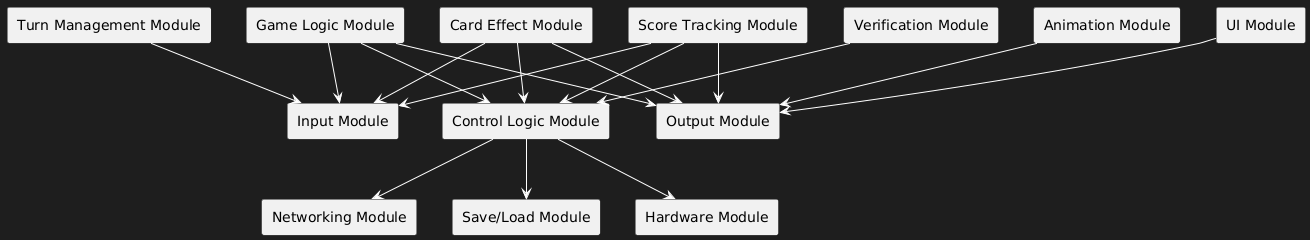
\includegraphics[width=0.7\textwidth]{output.png}
\caption{Use hierarchy among modules}
\label{FigUH}
\end{figure}


%\section*{References}

\section{User Interfaces}

The user interface (UI) design for this system focuses on creating an intuitive and accessible experience for players. The UI consists of both software and hardware elements that enable seamless interaction with the game. Below are the primary components of the UI design:

\subsection{Software User Interface}
\begin{itemize}
    \item \textbf{Main Menu:} The main menu provides options for starting a new game, loading a saved game, viewing instructions, and accessing settings.
    \item \textbf{Game Screen:} The game screen displays the game state, including player scores, active cards, and the current turn. Interactive elements allow players to perform actions such as playing a card or drawing from the deck.
    \item \textbf{Pop-Up Notifications:} Notifications are used to inform players about special events, such as a "Skip" card being played or a turn being reversed.
\end{itemize}

\subsection{Hardware User Interface}
\begin{itemize}
    \item \textbf{Input Devices:} Supports mouse, keyboard, and touchscreens for input.
    \item \textbf{Output Devices:} Designed for compatibility with various screen sizes and resolutions.
\end{itemize}



\section{Design of Communication Protocols}

The communication protocols in this system ensure reliable and efficient data exchange between modules, especially for multiplayer functionality. These protocols are designed to handle various aspects such as real-time data synchronization, error handling, and security.

\subsection{Protocol Overview}
\begin{itemize}
    \item \textbf{Transport Layer:} Uses WebSocket protocol for real-time communication in multiplayer games. Ensures low latency and high reliability.
    \item \textbf{Message Format:} Messages are serialized using JSON for simplicity and compatibility. Each message includes a header (e.g., message type) and a body (e.g., card played, turn updated).
\end{itemize}

\subsection{Error Handling and Recovery}
\begin{itemize}
    \item \textbf{Connection Loss:} Implements a reconnection mechanism to recover lost connections without disrupting the game state.
    \item \textbf{Invalid Messages:} Validates incoming messages to ensure compliance with the protocol specification. Invalid messages are logged and discarded.
\end{itemize}

\subsection{Security}
\begin{itemize}
    \item \textbf{Encryption:} All data exchanged between clients and the server is encrypted using TLS to ensure data security.
    \item \textbf{Authentication:} Players are authenticated via a token-based system to prevent unauthorized access.
\end{itemize}




\section{Timeline}

\wss{Schedule of tasks and who is responsible}

\wss{You can point to GitHub if this information is included there}

\begin{itemize}
    \item \textbf{January 20 – January 25: Project Planning and Requirements Gathering} \\
    Responsible: Jianhao Wei
    \item \textbf{January 26 – February 5: Game Core Development} \\
    Responsible: Zheng Bang Liang, Mingyang Xu
    \item \textbf{February 6 – February 12: User Interface Development} \\
    Responsible: Zain-Alabedeen Garada, Kevin Ishak
    \item \textbf{February 13 – February 20: Multiplayer and Network Functionality} \\
    Responsible: Mingyang Xu, Zain-Alabedeen Garada
    \item \textbf{February 21 – February 28: Integration and Initial Testing} \\
    Responsible: Jianhao Wei, Kevin Ishak
    \item \textbf{March 1 – March 10: Feedback and Feature Refinement} \\
    Responsible: Zheng Bang Liang, Zain-Alabedeen Garada
    \item \textbf{March 11 – March 20: Final Testing and Deployment} \\
    Responsible: Jianhao Wei, Mingyang Xu, Kevin Ishak
\end{itemize}


\bibliographystyle {plainnat}
\bibliography{../../../refs/References}
\begin{enumerate}
    \item D. L. Parnas, "On the Criteria to Be Used in Decomposing Systems into Modules," \textit{Communications of the ACM}, vol. 15, no. 12, pp. 1053--1058, 1972.
    \item C. Richardson, "Decompose by Subdomain," \textit{Microservices.io}, 2023.
    \item Stack Overflow, "Abstraction vs Information Hiding vs Encapsulation," \textit{Stack Overflow}, 2023.
    \item M. Xu, "UNO Flip 3D - SRS Volere Documentation," \textit{GitHub Repository}, 2023.
    \item M. Xu, "UNO Flip 3D - Software Architecture Document," \textit{GitHub Repository}, 2023.
\end{enumerate}

\newpage{}

\end{document}
